\section{Validation and Results}\label{sec:results}
This section introduces the results of performing fault injection with the \approach{} %fault injection 
tool. First, we show the steps of performing the fault injection, the variable parts, and the expected outcomes. Then, we show the real outcome, the performance of the PM framework and the detected bugs.

%Design and creation research methodology was selected for creating the fault injection approach. Design and creation methodology is used for investigating a certain phenomena by creating and designing a new artifact. The phenomena in this study is to test the robustness of the embedded distributed systems and the artifact is the fault injection approach.  

%Agile development process was utilized for creating the fault injection approach. Fault injection tool developed in four iterations. Random sending messages was implemented in the first iteration, then we integrated the random messages sending into the automatic testing environment in the second iteration. Messages delaying was implemented during the third iteration and was integrated into the automatic testing environment in the last iteration.  

As anticipated in the introduction, we developed the approach through an iterative approach. In order to evaluate if the fault injection approach reached the conformance level against its requirements, the approach was evaluated at the end of each iteration. 
%The evaluation was done by comparing the results of running the tool and the expected ones. 
At the end of the final iteration, we made a final validation. 
%conclusion was built on how well the approach worked. Final evaluation of the developed approach described at the result part in details, we could see that 
The fault injection approach has detected unexpected faults that were not found by previously used testing techniques. As matter of fact, we could also see that this approach is able to identify the bottleneck of existing embedded distributed systems.  In the following we report the detailed results of the validation. Specific information is however omitted according to a non disclosure agreement with the company.


\subsection{Sending random messages}
%The communication within the system follows some specific protocols.  Sending random messages is mainly developed to test the fault tolerance ability of the protocols. The messages are categorized into three types: request, confirmation, and rejection.  Based on the designed fault tolerance feature and the possible message types in reality, we only perform sending of random request messages. We focus on three aspects of the invalid messages, the origination, the contents and the amount of sending.
%
%The system is designed to tolerate invalid request messages, one main filtering standard of invalid messages is the origination of the messages. We focused on three aspects of the message origination, the namespace name, the mailbox name and combination of namespace and mailbox names. We first created multiple mailboxes which have the same namespace name, this means that the random messages are generated from different threads but the same process. Then we created mailboxes with same mailbox names but different namespace names; this means that the random messages are generated from both different threads and processes. Lastly, we created mailboxes with both different mailbox names and namespace names. Three cases of mailbox and namespace names are shown in Table~\ref{table:4.1}.
%
%\begin{table}[ht!]
%\centering
%\begin{tabular}{| c | c | c |r}
% \cline{1-3}
%       & mailbox & namespace \\ 
% \cline{1-3}
% case 1 & S & D & \hspace{1.3cm} S stands for same\\ 
% \cline{1-3}
% case 2 & D & S & D stands for different\\ 
% \cline{1-3}
% case 3 & D & D & \\ 
% \cline{1-3}
%\end{tabular}
%\caption{Combinations of mailbox and namespace names} %, S means same, D means different}
%\label{table:4.1}
%\end{table}
%
%The message contents inside the system varied dramatically: some contents describe the actual payload, some describe the protocol version, some specify the size of the messages. The fields of the messages were also different from each other. Based on the above characteristics, we constructed the random messages from two different aspects, random fields and random contents. 
%
%The amount of random messages would affect the filtering ability of the protocols. For instance, by sending one random message, the system is able to filter it, but by sending 1000 random messages, the system might only be able to filter 500 of them. With a huge amount of random messages, the CPU load of the systems would be high. Therefore, t
The validation related to injecting random messages aims to give an answer to this question: 

 \begin{itemize}
 \item {\em To what extent is the system able to filter invalid messages?} 
% \item {\em Does a high CPU load affect other parts of the system?} 
 \end{itemize}
 
 To answer the above question, we sent random messages in two ways, synchronously and asynchronously.
Filtering of invalid messages is conducted by checking the properties of the messages. Such checking consumes time and processing power. So the filtering ability can also be affected by the frequency of the random messages. To test the filtering ability of the PM framework in terms of random message frequencies, the random messages are sent to the PM framework with different frequencies. This was implemented by giving different time intervals between each message sending. 

The number of invalid messages that need to be generated in order to let the system behaves differently from what expected varies depending on the time interval between the messages as well as the time when the messages are triggered. Sending a lot of invalid messages without having any time interval between messages leads the system to behave differently than expected. This happens due to the fact that the computation power of the embedded components is limited, the number of the messages are large and there is not enough time between message sending. Thus, the system will not be able to recognize if a message is valid or not. 

\begin{figure}[h!]
\centering
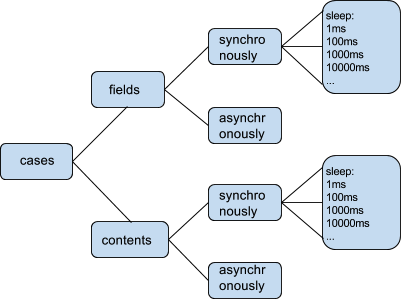
\includegraphics[width=.8\columnwidth]{figure/testingchain.png}
\caption{Testing chains \label{testingchain}}
\end{figure}

Figure~\ref{testingchain} shows the test chains of the PM framework. One sample test chain from the left to right can be read like this: test case1, with same fields but different contents, send the random messages synchronously, the time interval between each random message is 100ms. In order to perform the test randomly, we created different C++ classes to represent different variables in the chain. When the test starts, variable objects of the test chains are initialized and connected randomly. There are four variable classes, which are Cases, DataType (fields or contents), Concurrency (synchronously or asynchronously), and Intervals.

By performing the random message sending to the PM framework, we are able to test the PM framework according to two different aspects. The first aspect is the message type, which tested the PM framework at functional level. The second aspect is the message amount, which tested the PM framework at the performance level. The module test of the PM framework has covered almost all the invalid message sending, but the test is not random and the messages are sent one at a time. Our test sends random messages randomly and messages are also combined randomly. This helps the PM framework developers at Ericsson finding many corner cases that were not covered before. %which the module tested does not cover. 

Sending random messages also plays a performance test role. By adjusting the number of random messages and the time interval between the random messages sent, a performance threshold of the PM framework was found. Based on the demand in reality, this test helped the PM framework developers finding secure hardware requirements, which provide optimal and economic solutions for Ericsson.

\begin{figure}[h!]
\centering
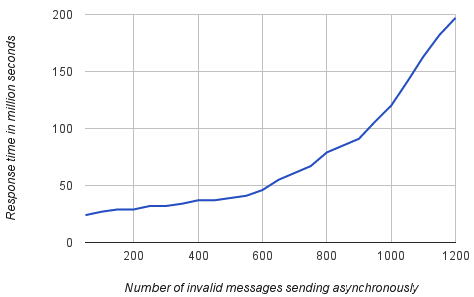
\includegraphics[width=\columnwidth]{figure/asynseding.png}
\caption{Sending invalid messages asynchronously \label{asynseding}}
\end{figure}

Figure~\ref{asynseding} shows a curve of sending random messages to one node in the PM framework. The response time of messages sent to this node should be less than 200 milliseconds. If no response is received after 200 milliseconds, the sender will time out. Figure~\ref{synchsending} shows a snapshot of sending random messages synchronously with different time intervals between each sending, which will not trigger timeout. Figure~\ref{asynseding} shows that the node can maximally receive 1200 random messages at the same time. Figure~\ref{synchsending} shows that in order to send 6000 messages, each message sending should have at least an interval of 80 milliseconds. These snapshots have been saved as benchmarks for improving the performance of the nodes.


\begin{figure}[hh!]
\centering
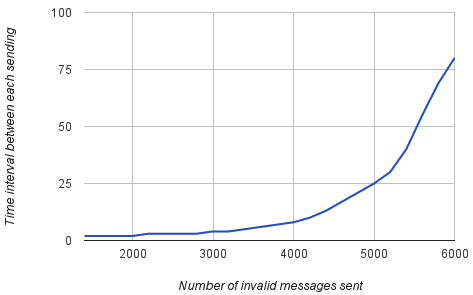
\includegraphics[width=\columnwidth]{figure/synchsending.png}
\caption{Sending invalid messages synchronously \label{synchsending}}
\end{figure}

Thanks to this tests we identified some errors that where not identified by traditional testing. For instance fuzzing of signals has detected a weakness in handling dynamically sized objects causing a crash which then could be rectified.

\subsection{Delaying messages}
%The second fault injection scenario was delaying the messages between the system components. The delay mechanism used default and randomize time interval between different components on the system in order to check if the system can handle different timeout intervals. There are multiple types of messages sending within the PM framework, e.g., request message, response message, rejection, confirmation message and messages describing the data. Some types of messages followed some time out mechanism strictly. For instance, when the connection request is sent, the node waits for confirmation or rejection messages for a period of time; if neither a confirmation nor a rejection message is received, the current request of the node just goes in timeout. 
%
%\begin{figure}[hh!]
%\centering
%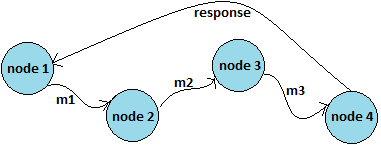
\includegraphics[width=.7\columnwidth]{figure/chaningMSG.png}
%\caption{Message delaying chain \label{chaning}}
%\end{figure}
%
%Some messages sent within the PM framework have relationships with each other. Those messages usually work as a chain, as shown in Figure~\ref{chaning}. In this case, \texttt{node1} sends a request to \texttt{node4} for some data, and at the same time a clock starts for the time out mechanism. In order to receive the data, some messages are sent to \texttt{node2} and \texttt{node3}, but \texttt{node1} only waits for a response from \texttt{node4}. Delaying can happen on any of the messages sent between \texttt{node1} and \texttt{node4}. In reality, such a chain can be really long and the delay of the messages sent between each nodes can also be very unpredictable.
%
%Delaying messages in the PM framework also tests the network performance of the framework. %By delaying messages in the PM framework, the network performance of the PM framework is tested. 
%Currently the PM framework network performance test is conducted by adjusting the network bandwidth. This approach has two main drawbacks. First, the test has some hardware requirements, which makes the test more complicated. Second, adjusting the network bandwidth makes the test uncontrolled, because the delaying of the message caused by a low network bandwidth is very hard to track. The current network performance test is like a black-box testing, since what is really going on in the system during the test is not peered. Our test provides a white box testing for the PM framework network performance. During the message delaying, each message delaying is recorded in the log file, and then the PM framework developers at Ericsson can easily track the message delaying. A future network bandwidth benchmark has been created based on the experiences of the message delaying.

In this case the validation aims to give an answer to the following question: 

 \begin{itemize}
 \item {\em Is delaying messages an effective strategy to discover faults?} 
 \end{itemize}

\begin{figure}[hh!]
\centering
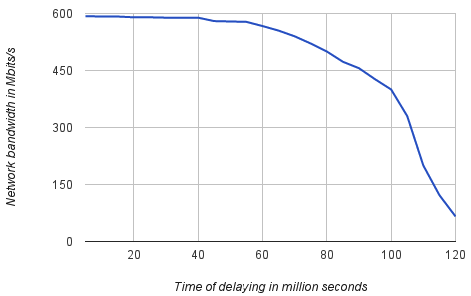
\includegraphics[width=\columnwidth]{figure/bendelay.png}
\caption{Message delaying and corresponding network bandwidth \label{bendelay}}
\end{figure}

In order to provide an answer to this question, we operated as follows. 
Figure~\ref{bendelay} shows the time of delaying in milliseconds and the corresponding network bandwidth in Mbit/s. The nodes use wireless communication and Ericsson uses the international standard of Wireless 802.11n~\cite{Wireless}, whose normal bandwidth is 600 Mbit/s. This benchmark is used to adjust the %when the performance test by adjusting 
network bandwidth when the performance is performing abnormally; the corresponding delaying will be run to check which process is responding slowly.

Randomized delays detect misconfigured time out handling. This was not identified by manual testing since the testers made the same wrong assumptions of the developers, %produced code, %manual test case had the same mistake of the production code, 
and consequently the defect was missed. This testifies the potential existence of human bias in manual testing.


